\documentclass[11pt]{beamer}

%%% \mode must be on a line by its own, without comment or whitespace!
%%% \mode sets the mode to presentation. So if the mode is presentation the slides after are shown
%%% if the mode is not presentation (but article or handout) they are not shown
\mode<presentation>

\usetheme{Warsaw}
\usepackage[utf8]{inputenc}
\usepackage[english]{babel}
\usepackage{amsmath}
\usepackage{amsfonts}
\usepackage{amssymb}
\usepackage{graphicx}
\usepackage{xspace}

\author{Guus Bonnema}
\title{Architecture}
%\setbeamercovered{transparent} 
%\setbeamertemplate{navigation symbols}{} 
%\logo{} 
\institute{Open University\\team033\\Guus Bonnema, Stefan Versluys, Jeroen Kleijn} 
\date{January 24, 2015} 
\subject{Progress iteration 1} 

\begin{document}

\newcommand{\Noc}{\textsc{NoC}\xspace}
\newcommand{\qt}{\textsc{Qt}\xspace}
\newcommand{\qml}{\textsc{Qml}\xspace}

\begin{frame}
\titlepage
\end{frame}

\begin{frame}
	\begin{itemize}
		\item Design using \qt  
		\item User Interface
		\item Data layer
		\item Open issues
	\end{itemize}
\end{frame}

\begin{frame}{Design using \qt}

	\begin{itemize}
		\item Use of regular graphics or \qml?
		\item Separation of concerns: data layer / presentation layer
		\item Integration of \qml and C++
		\item integration of features in VT plugin: DFS / BFS
	\end{itemize}

\end{frame}

\begin{frame}{User Interface}

	\begin{itemize}
		\item Stefan : demo
	\end{itemize}

\end{frame}

\begin{frame}{Data layer}

	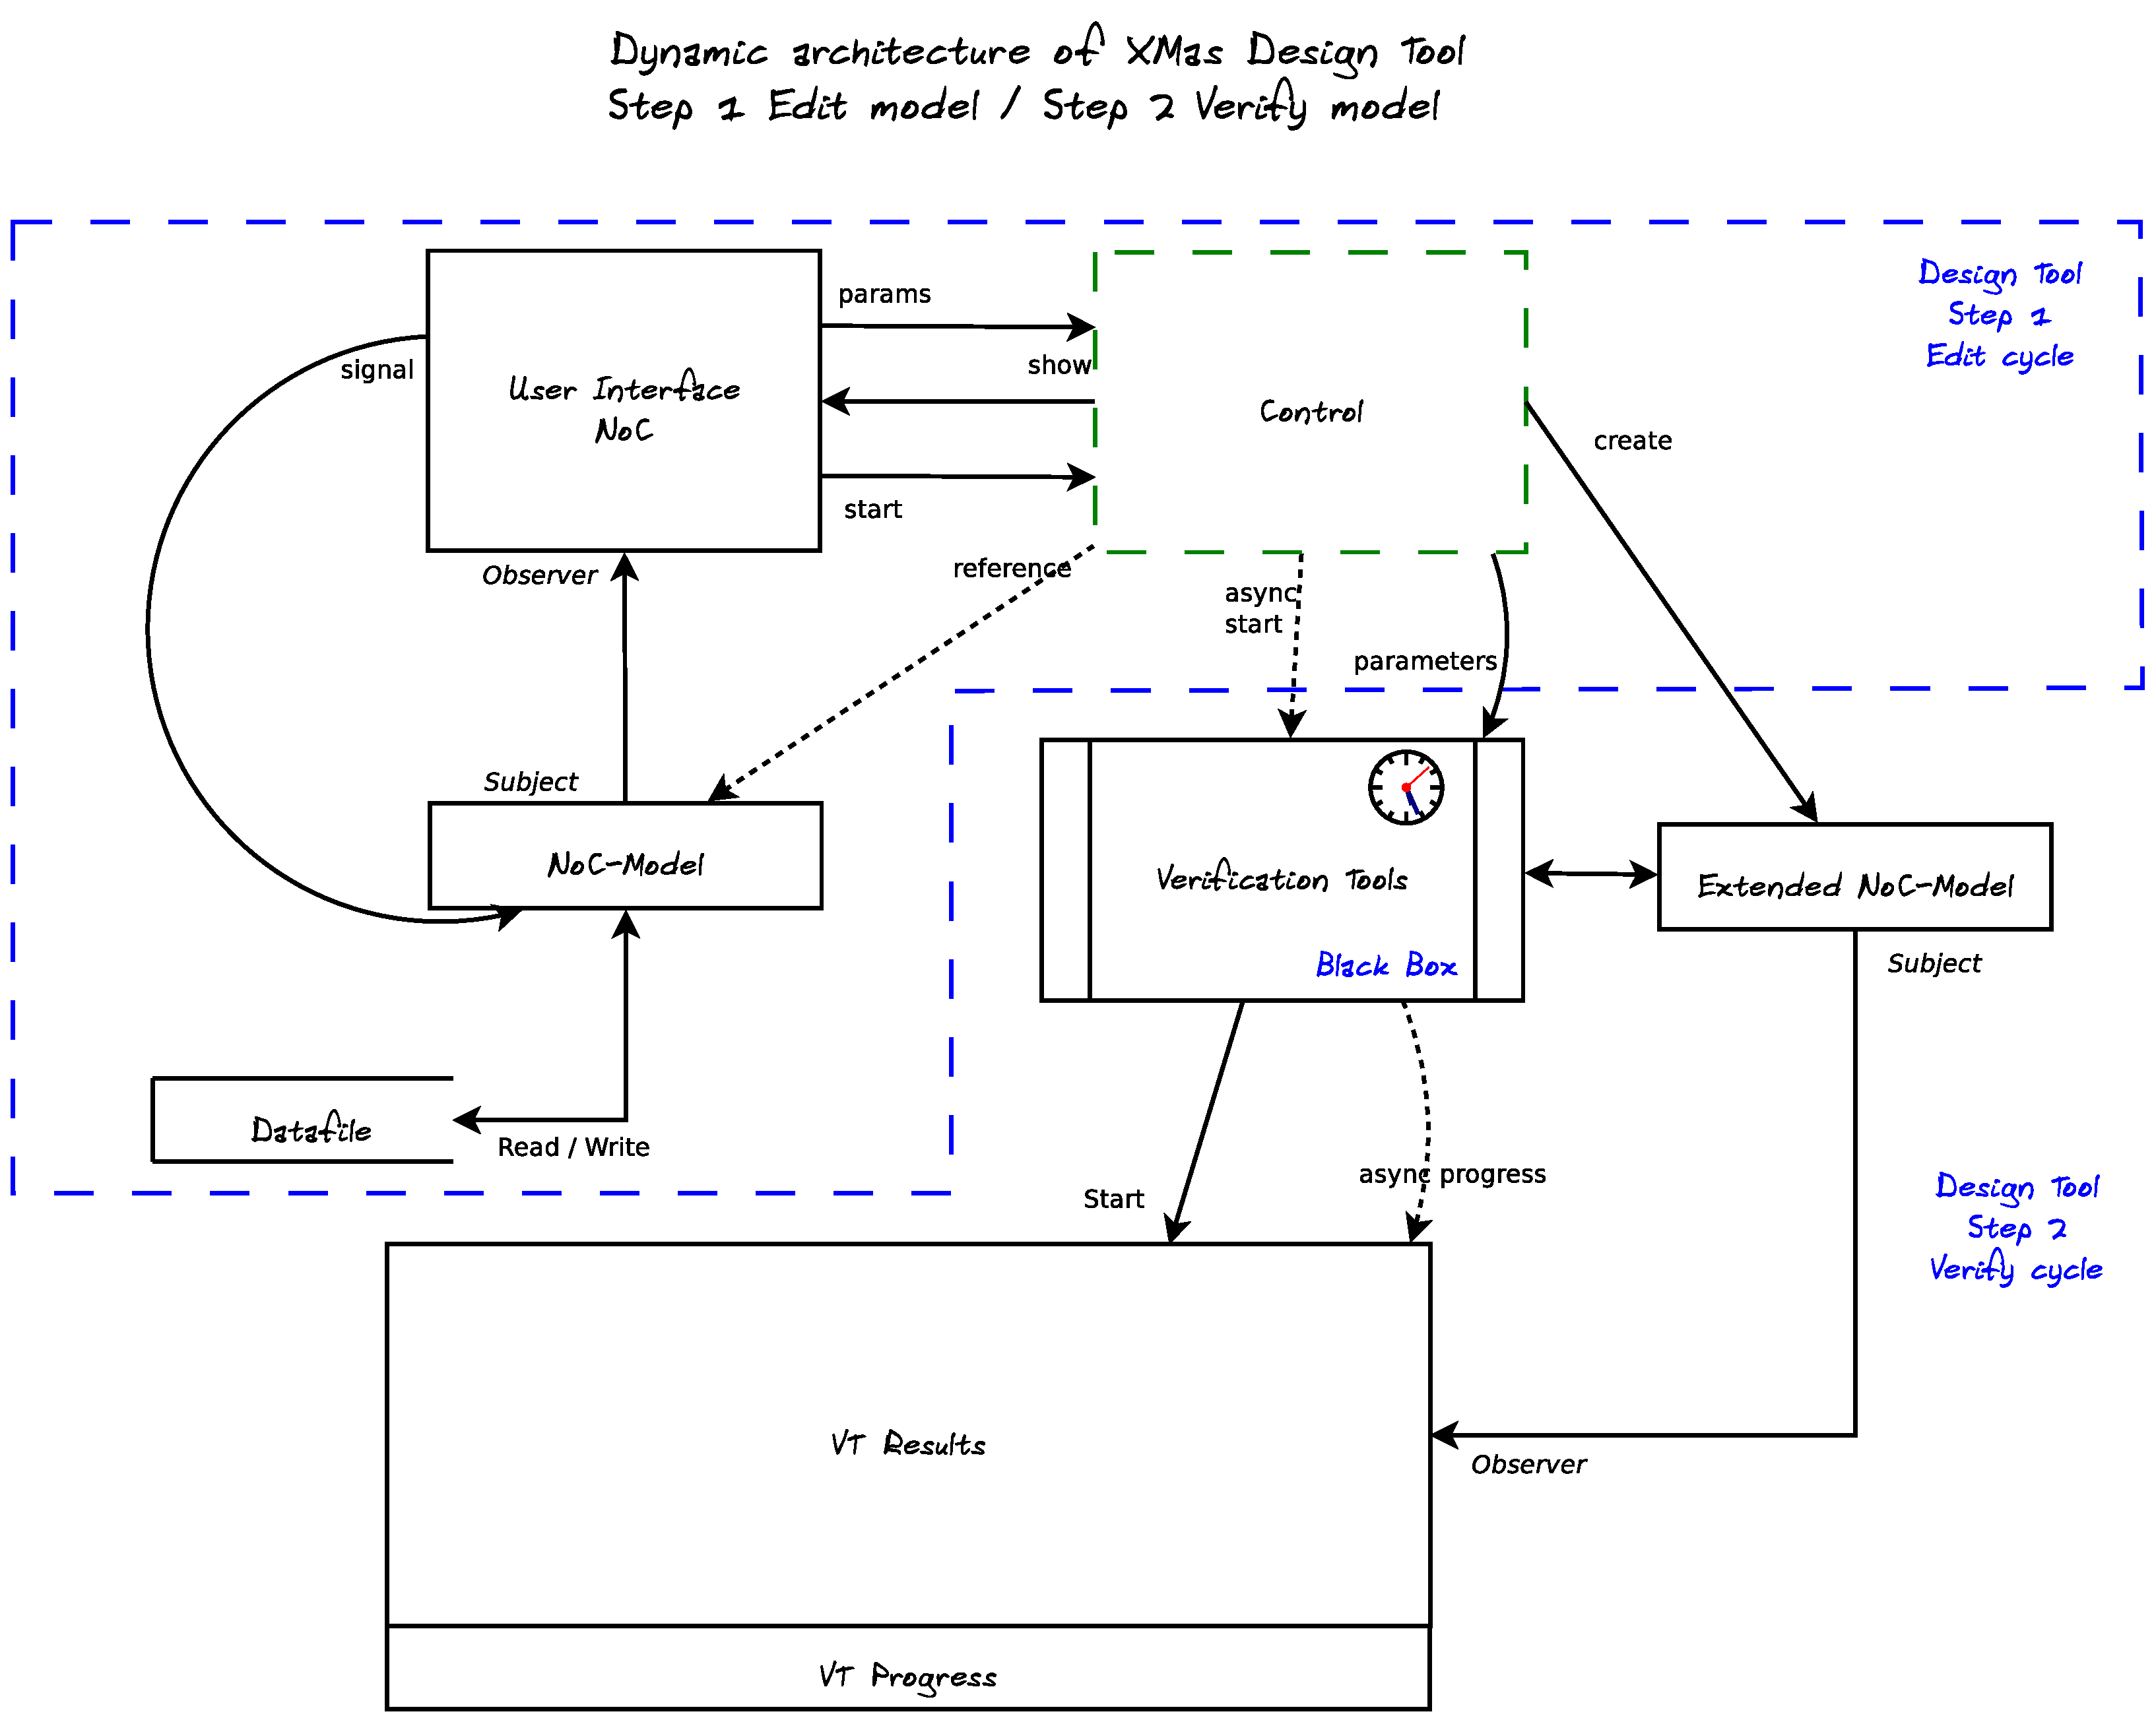
\includegraphics[width=.95\linewidth]{1c-architecture-dynamic}

\end{frame}

\begin{frame}{Data layer}

	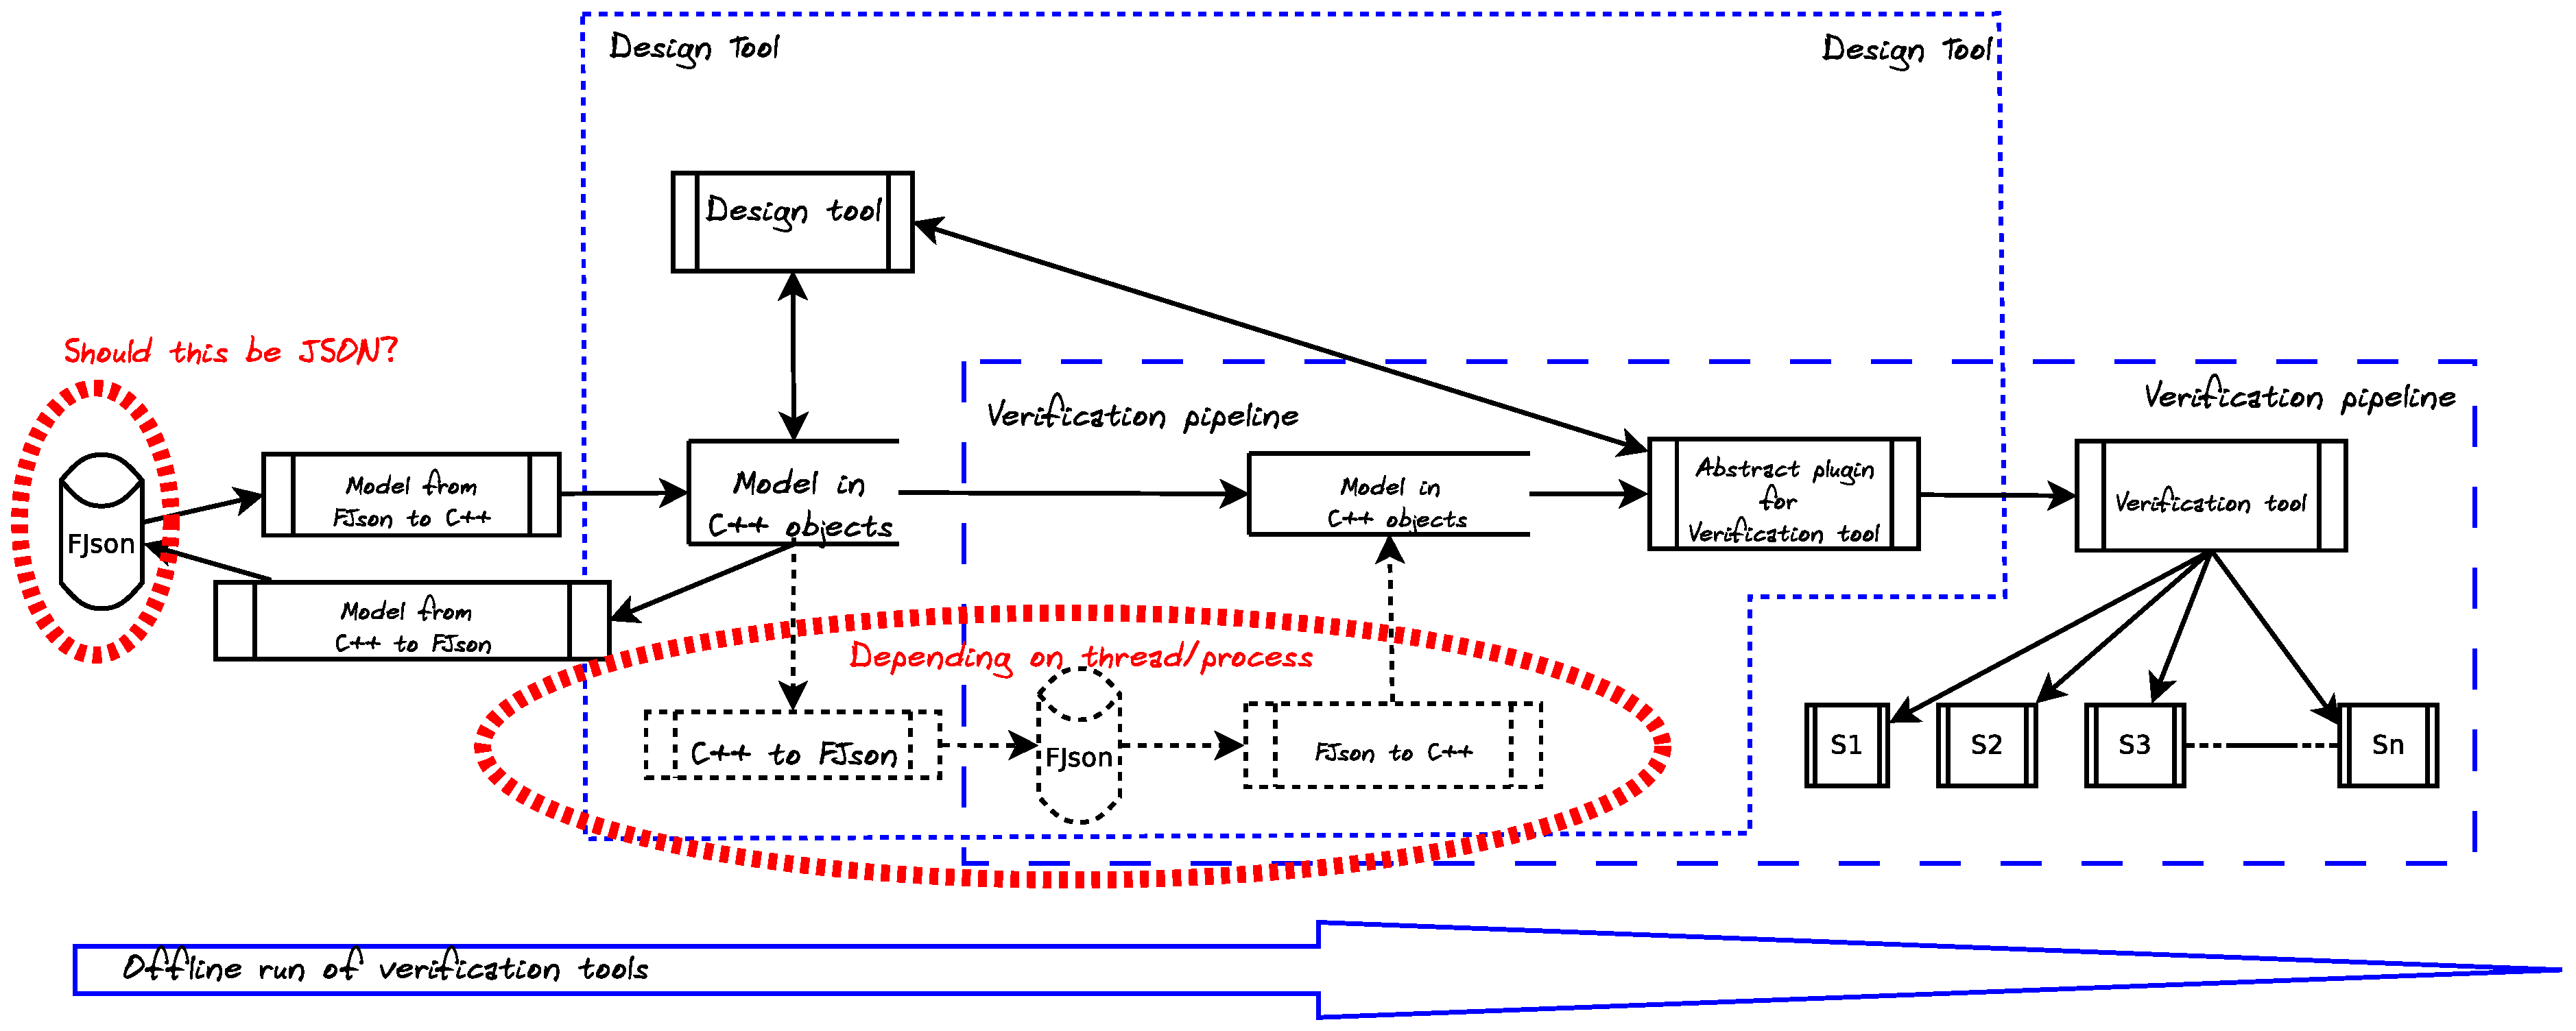
\includegraphics[width=.95\linewidth]{architecture-tool-scope}

\end{frame}

\begin{frame}{Open Issues}
	\begin{description}
		\item[data model - VT] How to integrate? Using Bernard's tools? 
		\item[dynamic checks] How tightly to integrate into designer
		\item[serialization] We can read QML,  but write?
		\item[Flat model] Are flat models still necessary?
		\item[Performance qml] How large will the networks be?
		\item[QML/js] Can we use recursive functions? (parametrised objects)
	\end{description}
\end{frame}

\end{document}
